\documentclass[10pt, conference]{IEEEtran}

\usepackage{float}
\usepackage{placeins}
\usepackage{graphicx}
\usepackage{subimages}
\setfigdir{figs}

\usepackage[cmex10]{amsmath}
\interdisplaylinepenalty=2500
\usepackage{amsthm}
\newtheorem{definition}{Definition}
\usepackage{hyperref}

\hyphenation{op-tical net-works semi-conduc-tor}

\graphicspath{{figs/}}
\begin{document}
	
	\title{Customer detection in shops using computer vision}
	
	%------------------------------------------------------------------------- 
	% change the % on next lines to produce the final camera-ready version 
	\newif\iffinal
	%\finalfalse
	\finaltrue
	\newcommand{\jemsid}{99999}
	%------------------------------------------------------------------------- 
	\author{%
		\IEEEauthorblockN{Nicolas A. Maduro}
		\IEEEauthorblockA{%
			Laboratory for Interdisciplinary Research on Multimedia Information\\
			CEFET-MG\\
			Belo Horizonte, Brazil\\
		}\and
		\IEEEauthorblockN{Thales B. Nascimento}
		\IEEEauthorblockA{%
			CEFET-MG\\
			Belo Horizonte, Brazil\\
		}
	}
	
	\maketitle
	
	\begin{abstract}
		This work presents a computer vision based system to detect clients on shops and help the analysis of their behavior. This information is valuable to shop owners and organizations, as it can be used to improve marketing strategies and use of available physical space. The proposed is a first step towards a complete system to detect, track and analyse customer behavior. Currently it is capable of detecting people in a static scene and generating heatmaps. Experimental results comparing manually made heatmaps and automatic ones produced by the application demonstrate it correctness.
	\end{abstract}
	
	\begin{IEEEkeywords}
		Heatmap; Background subtraction; Customer behavior;
		
	\end{IEEEkeywords}
	
	\IEEEpeerreviewmaketitle
	
	\section{Introduction}
	The analysis of behavior of clients in shops are of great value to shop owners and organizations, as it can be used to improve marketing strategies and use of available physical space. Some analysis of this kind made using computational tools currently impose some restrictions, for example requiring the client to use an RFID tag or even visual identifications in the products. Other tools are expensive to implement and therefore not well explored.
	
	This work implements a computer vision based system able to detect clients in shops in order to create heatmaps and help the client behavior analysis. We first filter the image using a Gaussian filter, then segment the image using background subtraction, producing a foreground that will be improved by morphological operations, and finally we accumulate the result to generate a heatmap.
	
	The remainder of this work is as follows: The second section presents the related work. The third section shows definitions of important concepts used in this work. The fourth section shows the proposed approach to solve the problem. The next section exposes the experimental results and the last section finishes with concluding remarks.
	
	\subsection{Contribution}
	The contribution of this work is to present a simple method to detect people in an store environment and provide a heatmap to help understanding the client behavior in real time.
	
	\section{Related work}
	The work of Padua~\cite{padua2014sistema} is a computer vision based system designed to help tactical and physical analysis on indoor soccer. In this system were used Gaussian mixture based background subtraction\cite{zivkovic2004improved} and morphological opening and closing\cite{haralick1987image} on the foreground in order to detect players. He further processes the data data to track and generate measures for each player.
	
	Liciotti et al~\cite{liciotti2014shopper} presents an integrated system consisted of a RGB-D camera and software able to monitor shoppers behavior and their interactions with products in shelves. Their system univocally identifies people within a store, and by using depth information it determines the kind of action the shopper is taking on the products, either touching, picking up or putting back.
	
	Popa et al.~\cite{popa2013semantic} approaches the possibility of automatic understanding of customers’s shopping behavior. From the video recordings, they extract features related to the spatio-temporal behavior of customers, like dynamics and time spent in each region of interest and customer-products interaction patterns. Then they analyze the shopping sequences using a Hidden Markov Model. They got accurately classify trajectories (93\%), discriminate between different shopping related actions (91.6\%), and recognize shopping behavioral types by means of the proposed reasoning model in 95\% of the cases.
	
	Haritaoglu and Myron~\cite{haritaoglu2001detection} create a monocular real-time computer vision system that identifies shopping groups by detecting and tracking multiple people as they wait in a checkout line or service counter. The system segments each frame into foreground regions which contains multiple people. Those are further segmented into individuals using a temporal segmentation and motion cues. Once a person is detected, an appearance model based on color, edge density and mean-shift tracker is used to recover the person’s trajectory. People are grouped together as a shopping group by analyzing interbody distances. The system also monitors cashier’s activities to determine when shopping transactions start and end.
	
	Breitenstein~\cite{breitenstein2011online} proposes an approach for multi-person tracking in a particle filtering framework. It combines online trained, instance-specific classifiers with generic object category knowledge, resulting in a robust multi-person tracking. The algorithm detects and tracks a large number of dynamically moving persons in complex scenes with occlusions, without relying in background models or camera calibration, using only information from the past, hence imposing very few restrictions and is suitable for online applications.
	
	All the above mentioned works, except Breitenstein's, use some kind of foreground detection to segment the input image. The technique is well studied and for that reason we used the same approach in this work.
	
	\section{Fundamentals}
	In this section we present some important concepts used in our algorithm.
	\begin{definition}[Image binarization]
		Binarization is the conversion of a gray scale image to a two values image. There are many binarization formulas, we used the following:
		\[
		output(x,y) =
		\begin{cases}
		G_{max} & \text{if } input(x,y) > \text{threshold}\\
		0 & \text{otherwise}
		\end{cases}.
		\]
	\end{definition}
	\begin{definition}[Gaussian filter]
		The Gaussian Filter is a 2D convolution with a kernel defined by samples of the 2D Gauss function. This function is defined as follows:
		$$ G_{\sigma,\mu_{x},\mu_{y}}(x,y)=\frac{1}{2\pi\sigma^{2}}
		e^{\frac{(x-\mu_{x})^{2}}{2\sigma^{2}}}
		e^{\frac{(y-\mu_{y})^{2}}{2\sigma^{2}}}.$$
		
	\end{definition}
	\begin{definition}[Morphological Dilation]
		Dilation is the morphological transformation which combines two sets using vector addition of set elements. Let A and B be subsets of image carrier $\Omega$. The dilation is defined as: $$A \oplus B=\{c\in\Omega|c=a+b \text{ for some }a\in A\text{  and }b \in B\}.$$
	\end{definition}
	
	\begin{definition}[Morphological Erosion]
		Erosion is the morphological dual to dilation.Let A and B be subsets of image carrier $\Omega$. The erosion is defined as: $$A \ominus B=\{x\in\Omega | x+b \in A \text{ for every }b\in B.$$
	\end{definition}
	
	\begin{definition}[Morphological Opening]
		The opening of image $B$ by structuring	element $K$ is denoted by $B \circ K$ and is defined as: $$B \circ K =(B \ominus K) \oplus K.$$
	\end{definition}
	
	\begin{definition}[Morphological Closing]
		The closing of image $B$ by structuring	element $K$ is denoted by $B \circ K$ and is defined as: $$B \circ K =(B \oplus K) \ominus K.$$
	\end{definition}
	
	\begin{definition}[Background subtraction]
		Background subtraction (BS) is a technique used for detecting moving objects in videos from static cameras. It calculates the foreground performing a subtraction between the current frame and a background model, which contains everything that can be considered as background.
	\end{definition}
	
	\section{Proposed Approach}
	In order to detect people in the scene we follow scheme described in \autoref{diagramablocos}.
	\begin{figure}[H]
		\centering
		\includegraphics[height=12cm]{diagrama_blocks}
		\caption{Block diagram of the system.}
		\label{diagramablocos}
	\end{figure}
	
	
	\subsection{Gaussian filter}
	For each frame of the input video we use a Gaussain filter to reduce noise. This filter produces an output image blurrier than the original image, as exemplified on \autoref{filterexample}. As we are not interested on small details, this effect has no relevance.
	\begin{figure}[H]
		\includegraphics[width=0.5\textwidth]{filterexample}
		\centering
		\caption{Example of an application of a Gaussian filter on the left image}
		\label{filterexample}
	\end{figure}
	\subsection{Background subtraction}
	With each filtered frame, the system perform a background subtraction in order to segment the image and detect people in the scene. While there are many BS implementations, our application demands an adaptive technique that is able to update its background model when the scene changes permanently, for example when a customer removes a product from the shelve. For that reason, we used the BS technique proposed by Zivkovic~\cite{zivkovic2004improved}, which is implemented in OpenCV~\cite{opencv_library}. \autoref{bgexample} shows an example of the technique.
	\begin{figure}[H]
		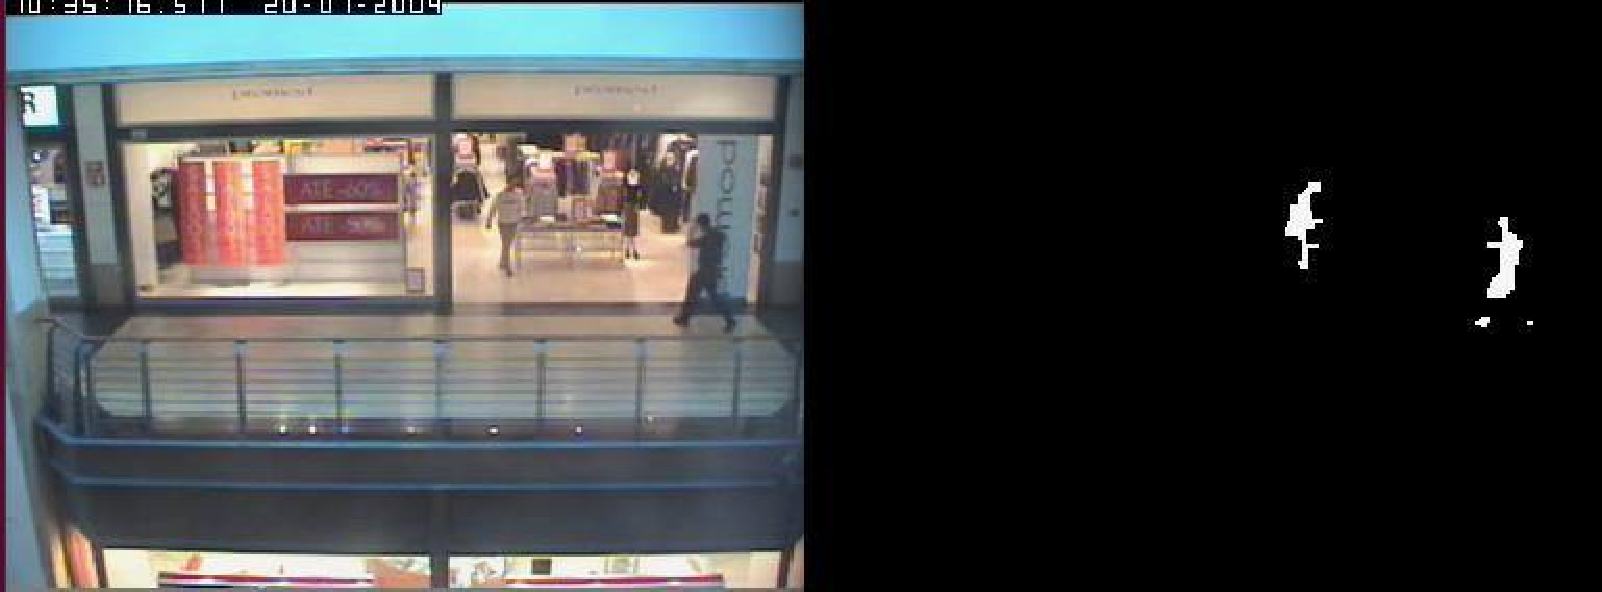
\includegraphics[width=0.5\textwidth]{figs/bgexample}
		\centering
		\caption{example of a background subtraction. The the algorithm was applied on the left image to produce the right one}
		\label{bgexample}
	\end{figure}
	\subsection{Threshold}
	The BS implementation we used deliver an image with the shadow pixels marked in gray, while the foreground is marked in white. The shadows are of no interest to our application, so they are removed with a threshold operation. The results of this step can be seen in \autoref{binarizationexample}.
	\begin{figure}[H]
		\centering
		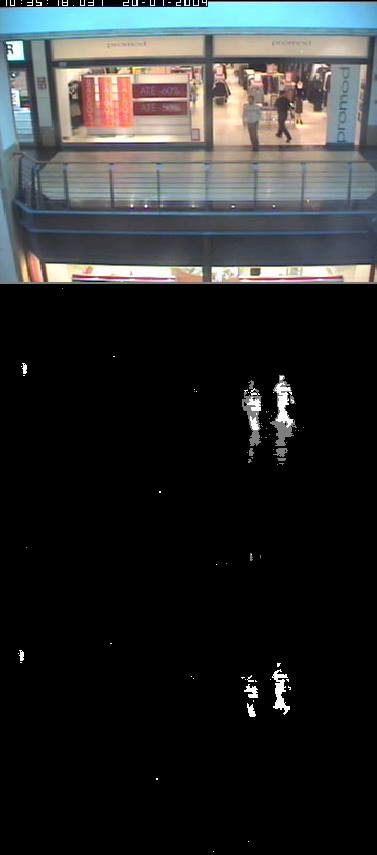
\includegraphics[height=0.5\textheight]{figs/binarizationexample}
		\caption{Comparation of two images after(right) and before(left) morphological transformation}
		\label{binarizationexample}
	\end{figure}
	
	\subsection{Morphological opening and closing}
	In order to improve the foreground representation, we apply morphological opening and closing\cite{haralick1987image} in the output of the threshold step. The first is used to remove small noise from the image, while the second is used to remove small holes on the detected objects. A comparative of a foreground before and after the application is show in \autoref{morphologicalexample};
	\begin{figure}[H]
		\centering
		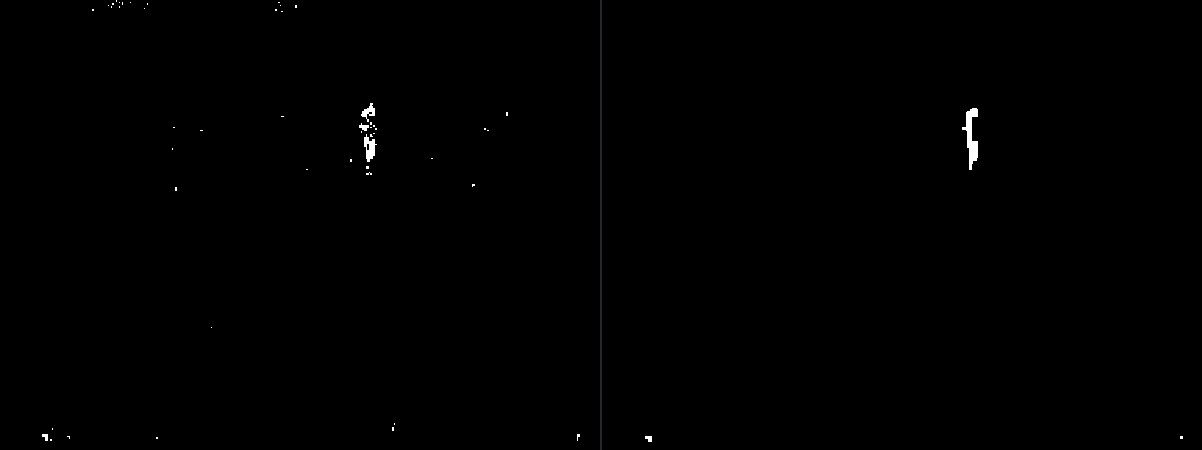
\includegraphics[width=0.5\textwidth]{figs/morphological}
		\caption{Comparation of two images after(right) and before(left) morphological transformation}
		\label{morphologicalexample}
	\end{figure}
	
	\subsection{Accumulation}
	In this step we add the result of previous operation in an accumulator, for further generating a heatmap.
	
	\subsection{Normalization and display}
	If all frames were computed, the accumulator matrix is normalized in order to be in a displayable format \textit{i.e.} between 0 and 1, and then it is colorized for better viewing with one of the colorscales show in \autoref{colorscaleexample}. One example of heatmap is showed in \autoref{heatmapexample}.
	\begin{figure}[H]
		\centering
		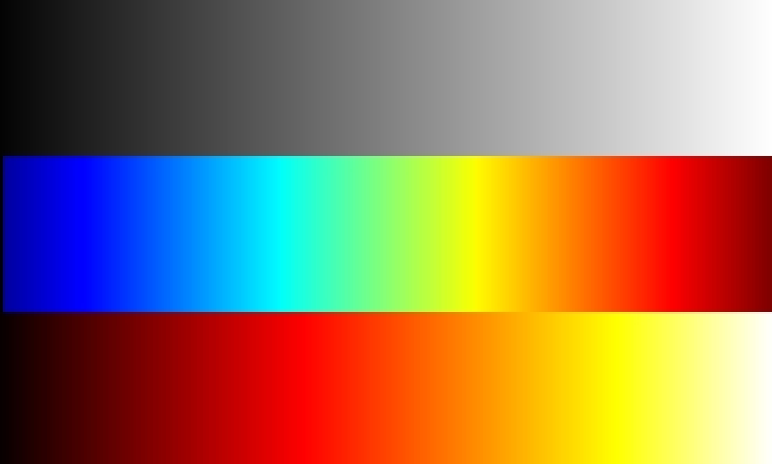
\includegraphics[width=0.5\textwidth,height=0.05\textheight]{figs/colorscaleexample}
		\caption{colorscales jet (middle) and hot (bottom)}
		\label{colorscaleexample}
	\end{figure}
	\begin{figure}[H]
		\centering
		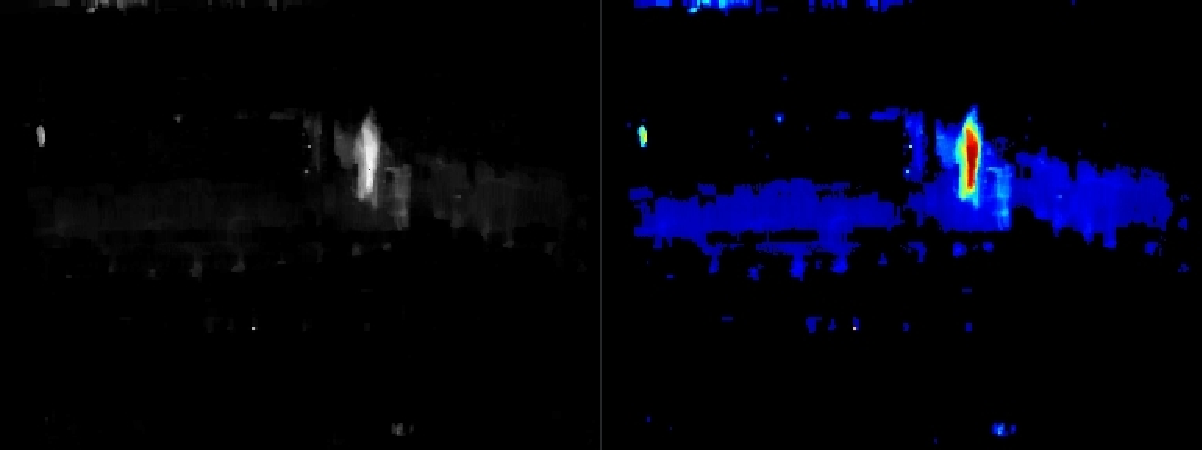
\includegraphics[width=0.5\textwidth]{figs/heatmapexample}
		\caption{Example of a heatmap produced by the algorithm. Both images represent the same heatmap, left in grayscale and right in jet colorscale}
		\label{heatmapexample}
	\end{figure}
	
	
	\section{Experimental results}
	In order to verify the correctness of the algorithm, it was designed an manual heatmap builder. For each frame, the user has to mark the persons on the frame, and the application generates a heatmap based on the user marks on all frames. The process can be seen in \autoref{manualshow}. The dataset used for the experiments was CAVIAR\footnote{http://homepages.inf.ed.ac.uk/rbf/CAVIARDATA1/}.
	\begin{figure}[H]
		\centering
		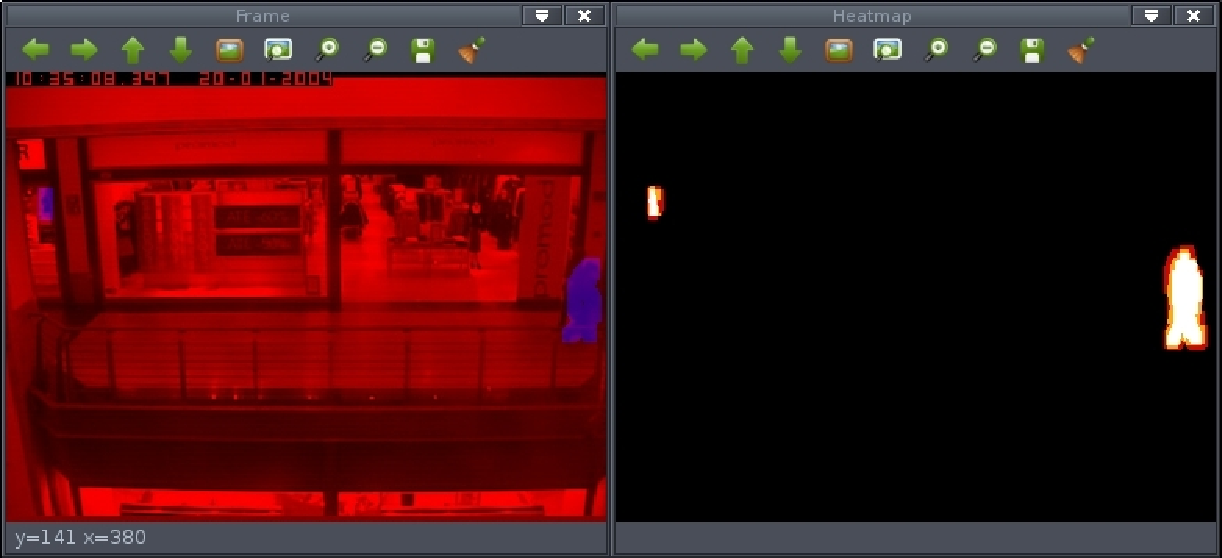
\includegraphics[width=0.5\textwidth]{figs/manualshow}
		\caption{User interface of the application used to generate a manual heatmap. On the right is the current heatmap, on left are the frame intensity on the red channel, and the user overlay on blue channel}
		\label{manualshow}
	\end{figure}
	A comparation of the manual and automatic generated result is show in \autoref{comparacaoheatmaps}. \autoref{redondo} shows the same comparison, but with a base video from a fish eye camera. We can see that there are differences, but the overall result is close, which validate our algorithm.
	\begin{figure}[H]
		\centering
		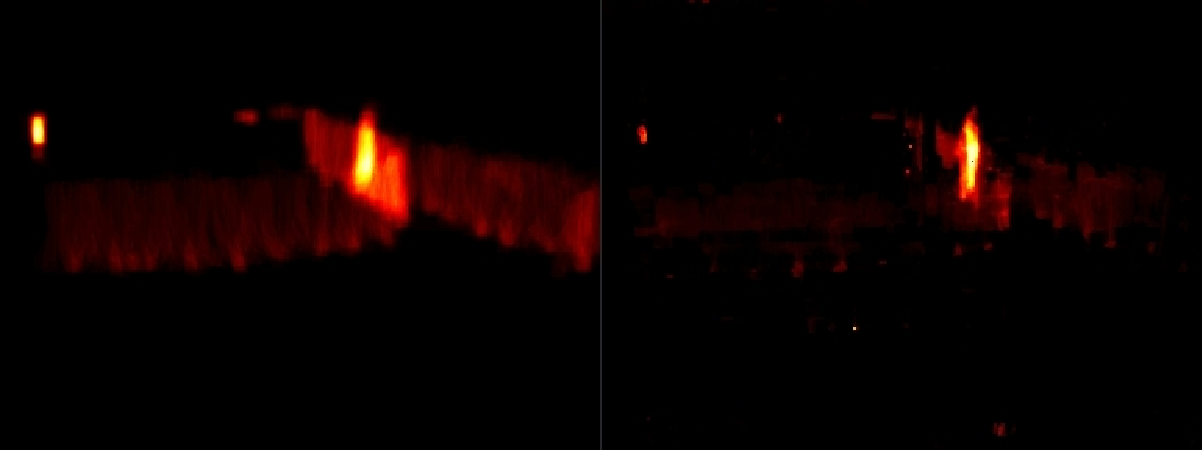
\includegraphics[width=0.5\textwidth]{figs/comparacaoheatmaps}
		\caption{Comparation of the manual(left) and automatic(right) heatmaps}
		\label{comparacaoheatmaps}
	\end{figure}
	\begin{figure}[H]
		\centering
		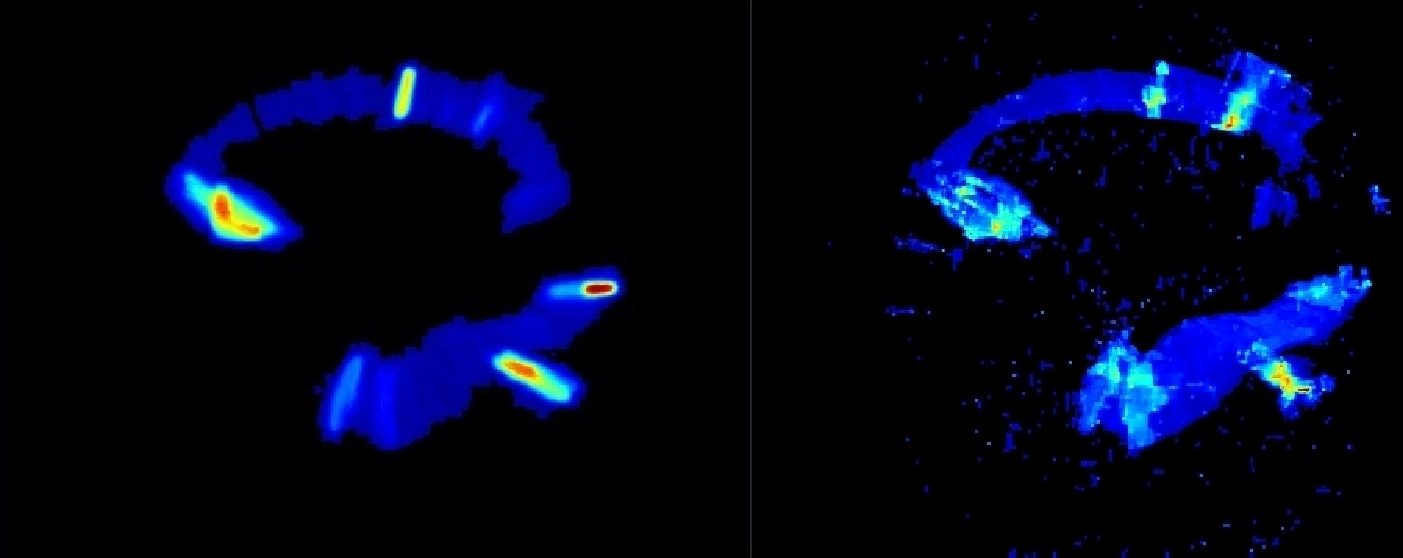
\includegraphics[width=0.5\textwidth]{figs/redondo}
		\caption{Comparation of the manual(left) and automatic(right) heatmaps created from a fish eye camera video}
		\label{redondo}
	\end{figure}
	
	\section{Concluding Remarks}
	The algorithm produces results coherent to the ground truth, in real time. With this work we were able to obtain a metric important to the analysis of videos of customers on shops. This is the first step, to construct a complete, automatic system, capable of not only detecting, but also tracking and identifying interactions of clients, and then generate important statistics.
	
	\section*{Acknowledgment}
	The authors would like to thank Flavio Cardeal for his course and support on this work.
	
	% trigger a \newpage just before the given reference
	% number - used to balance the columns on the last page
	% adjust value as needed - may need to be readjusted if
	% the document is modified later
	%\IEEEtriggeratref{8}
	% The "triggered" command can be changed if desired:
	%\IEEEtriggercmd{\enlargethispage{-5in}}
	
	\bibliographystyle{IEEEtran}
	\bibliography{example}
	
\end{document}
